% !TeX program = xelatex
\documentclass[aspectratio=169, 10pt, xcolor={x11names}]{beamer}

\usepackage{amsmath, amssymb, mathtools}
\usepackage{array}
\usepackage{booktabs}
\usepackage{multirow}
\usepackage{graphicx}
\usepackage{tikz}

\usetikzlibrary{arrows.meta, calc, positioning}

% --- Palette: Navy + Amber Gold (matched to report) ---
\definecolor{primary}{RGB}{28, 55, 90}
\definecolor{accent}{RGB}{176, 128, 52}
\definecolor{accentlight}{RGB}{232, 214, 178}
\definecolor{progcolor}{RGB}{52, 105, 88}
\definecolor{textmuted}{RGB}{95, 105, 118}
\definecolor{softbg}{RGB}{250, 248, 243}
\definecolor{coverbg}{RGB}{252, 249, 238}

\usetheme{Madrid}
\usecolortheme{default}

\setbeamercolor{structure}{fg=primary}
\setbeamercolor{palette primary}{bg=primary, fg=white}
\setbeamercolor{palette secondary}{bg=accent, fg=white}
\setbeamercolor{palette tertiary}{bg=primary!90!black, fg=white}
\setbeamercolor{title}{fg=primary}
\setbeamercolor{subtitle}{fg=accent}
\setbeamercolor{frametitle}{bg=primary, fg=white}
\setbeamercolor{block title}{bg=primary, fg=white}
\setbeamercolor{block body}{bg=softbg, fg=black}
\setbeamercolor{block title alerted}{bg=accent, fg=white}
\setbeamercolor{block body alerted}{bg=accent!10, fg=black}
\setbeamercolor{block title example}{bg=progcolor, fg=white}
\setbeamercolor{block body example}{bg=progcolor!8, fg=black}
\setbeamercolor{itemize item}{fg=accent}
\setbeamercolor{itemize subitem}{fg=primary}
\setbeamercolor{enumerate item}{fg=primary}
\setbeamertemplate{navigation symbols}{}
\setbeamertemplate{enumerate items}[default]
\setbeamertemplate{itemize items}[circle]

\setbeamertemplate{footline}{%
  \leavevmode%
  \hbox{%
    \begin{beamercolorbox}[wd=.42\paperwidth,ht=2.4ex,dp=1ex,left,leftskip=1.2em]{author in head/foot}%
      \usebeamerfont{author in head/foot}\textsf{ADS Project 1: Compare Search Trees}
    \end{beamercolorbox}%
    \begin{beamercolorbox}[wd=.38\paperwidth,ht=2.4ex,dp=1ex,center]{title in head/foot}%
      \usebeamerfont{title in head/foot}\textsf{\insertsectionhead}
    \end{beamercolorbox}%
    \begin{beamercolorbox}[wd=.20\paperwidth,ht=2.4ex,dp=1ex,right,rightskip=1.2em]{date in head/foot}%
      \usebeamerfont{date in head/foot}\textsf{\insertframenumber\,/\,\inserttotalframenumber}
    \end{beamercolorbox}%
  }%
  \vskip0pt%
}

% --- Automatic Section Transition Divider Pages ---
\AtBeginSection[]{
  \begin{frame}[plain]
    \begin{tikzpicture}[remember picture, overlay]
      \fill[coverbg] (current page.south west) rectangle (current page.north east);
      \fill[primary] (current page.north west) rectangle ([yshift=-0.22cm]current page.north east);
      \fill[accent] ([yshift=-0.22cm]current page.north west) rectangle ([yshift=-0.30cm]current page.north east);
      \draw[accent!45, line width=0.7pt]
        ([xshift=1.1cm, yshift=-1.1cm]current page.north west) --
        ([xshift=1.1cm, yshift=1.1cm]current page.south west);
      \draw[accent!45, line width=0.7pt]
        ([xshift=-1.1cm, yshift=-1.1cm]current page.north east) --
        ([xshift=-1.1cm, yshift=1.1cm]current page.south east);
      \foreach \r in {1.6, 2.0, 2.4} {
        \draw[primary!12, line width=0.5pt]
          ([xshift=-1.1cm, yshift=1.1cm]current page.south east) circle (\r cm);
      }
    \end{tikzpicture}
    \vfill
    \begin{center}
      {\normalsize\bfseries\color{accent}\textsf{SECTION \thesection}}\\[0.35cm]
      {\color{primary}\rule{0.35\textwidth}{1.2pt}}\\[0.45cm]
      {\LARGE\bfseries\color{primary}\insertsectionhead}\\[0.45cm]
      {\color{accent}\rule{0.18\textwidth}{0.9pt}}\\[0.65cm]
      \begin{minipage}{0.68\textwidth}
        \small\tableofcontents[currentsection, hideothersubsections]
      \end{minipage}
    \end{center}
    \vfill
  \end{frame}
}

% --- Helper Macros ---
\newcommand{\code}[1]{\texttt{\color{primary!90!black}#1}}
\newcommand{\bfactor}[1]{\ensuremath{\mathrm{BF}(#1)}}
\newcommand{\kw}[1]{\textbf{\color{primary}#1}}
\newcommand{\id}[1]{\ensuremath{\mathrm{#1}}}

\tikzset{
    avlnode/.style={circle, draw=primary, very thick, fill=primary!8, minimum size=6.2mm, inner sep=0pt, font=\scriptsize\bfseries, text=primary},
    avledge/.style={-{Stealth[length=1.8mm]}, thick, primary},
    rbblack/.style={circle, draw=primary!95!black, very thick, fill=primary!90!black, minimum size=4.8mm, inner sep=0pt, font=\tiny\bfseries, text=white},
    rbred/.style={circle, draw=Red3, very thick, fill=Red3!14, minimum size=4.8mm, inner sep=0pt, font=\tiny\bfseries, text=Red3!90!black},
    rbany/.style={circle, draw=accent!90!black, very thick, fill=accent!22, minimum size=4.8mm, inner sep=0pt, font=\tiny\bfseries, text=primary},
    rbdouble/.style={circle, draw=primary!95!black, double=white, double distance=0.9pt, very thick, fill=primary!90!black, minimum size=4.8mm, inner sep=0pt, font=\tiny\bfseries, text=white}
}

\graphicspath{{../src/visualizations/}}

\title[Compare Search Trees]{Performance Comparison and Analysis of Search Trees}
\subtitle{Advanced Data Structures and Algorithm Analysis $\cdot$ Project 1}
\author[Yixiang Chen, Runhui Lin]{Yixiang Chen \hspace{2em} Runhui Lin}
\institute[Zhejiang University]{School of Mathematical Sciences, Zhejiang University}
\date{2026-10-19}

\begin{document}

% ============================================================
%  COVER SLIDE
% ============================================================
\begin{frame}[plain]
\begin{tikzpicture}[remember picture, overlay]
    \fill[coverbg] (current page.south west) rectangle (current page.north east);
    \fill[primary] (current page.north west) rectangle ([yshift=-0.25cm]current page.north east);
    \fill[accent] ([yshift=-0.25cm]current page.north west) rectangle ([yshift=-0.34cm]current page.north east);
    \draw[accent!45, line width=0.7pt]
        ([xshift=1.1cm, yshift=-1.0cm]current page.north west) --
        ([xshift=1.1cm, yshift=1.0cm]current page.south west);
    \draw[accent!45, line width=0.7pt]
        ([xshift=-1.1cm, yshift=-1.0cm]current page.north east) --
        ([xshift=-1.1cm, yshift=1.0cm]current page.south east);
    \foreach \r in {1.6, 2.0, 2.4} {
        \draw[primary!14, line width=0.5pt]
            ([xshift=-1.1cm, yshift=1.0cm]current page.south east) circle (\r cm);
        \draw[primary!14, line width=0.5pt]
            ([xshift=1.1cm, yshift=-1.0cm]current page.north west) circle (\r cm);
    }
\end{tikzpicture}

\vspace*{0.55cm}
\begin{center}
    {\small\color{accent}\textsf{\textbf{Advanced Data Structures and Algorithm Analysis}}}\\[0.12cm]
    {\footnotesize\color{textmuted}\textsf{Laboratory Project Presentation $\cdot$ Project 1}}\\[0.35cm]
    {\color{primary}\rule{0.58\textwidth}{1.2pt}}\\[0.32cm]
    {\LARGE\bfseries\color{primary} Performance Comparison and}\\[0.12cm]
    {\LARGE\bfseries\color{primary} Analysis of Search Trees}\\[0.28cm]
    {\color{accent}\rule{0.22\textwidth}{0.9pt}}\\[0.45cm]
    {\normalsize\bfseries\color{primary} Yixiang Chen \hspace{2.5em} Runhui Lin}\\[0.18cm]
    {\footnotesize\color{textmuted} School of Mathematical Sciences, Zhejiang University}\\[0.1cm]
    {\scriptsize\color{textmuted} Fall--Winter 2026}
\end{center}
\end{frame}

% ============================================================
%  OUTLINE
% ============================================================
\begin{frame}{Presentation Outline}
\begin{columns}[T,onlytextwidth]
\begin{column}{0.48\textwidth}
\begin{block}{Part I: Specification \& Design}
\begin{itemize}\setlength{\itemsep}{0.55em}
  \item \textbf{Introduction}
  \begin{itemize}\footnotesize
    \item Five Search Tree Families
    \item Three Benchmark Workloads ($N \le 50{,}000$)
  \end{itemize}
  \item \textbf{Data Structure \& Algorithm Specification}
  \begin{itemize}\footnotesize
    \item Node Layouts \& Iterative Unbalanced BST
    \item AVL Tree, Splay Tree, Red-Black Tree, $\text{B}^+$ Tree
  \end{itemize}
\end{itemize}
\end{block}
\end{column}
\begin{column}{0.48\textwidth}
\begin{exampleblock}{Part II: Experiments \& Analysis}
\begin{itemize}\setlength{\itemsep}{0.55em}
  \item \textbf{Testing Results}
  \begin{itemize}\footnotesize
    \item Functional Verification \& Graphviz Topologies
    \item Benchmark Timings \& Runtime Curves
  \end{itemize}
  \item \textbf{Analysis and Comments}
  \begin{itemize}\footnotesize
    \item Time \& Space Complexity Comparison
    \item Three Key Empirical Findings \& Optimizations
  \end{itemize}
\end{itemize}
\end{exampleblock}
\end{column}
\end{columns}
\end{frame}

% ============================================================
%  SECTION 1: INTRODUCTION
% ============================================================
\section{Introduction}

\subsection{Search Tree Families and Benchmark Workloads}
\begin{frame}{Problem Statement \& Five Search Tree Families}
\begin{itemize}\setlength{\itemsep}{0.4em}
  \item \textbf{Goal:} Implement, verify, and benchmark \textbf{5 search tree structures} in C across $N \in [1{,}000, 50{,}000]$ distinct integer keys.
\end{itemize}

\vspace{0.3em}
\begin{block}{Five Candidate Structures}
\begin{itemize}\setlength{\itemsep}{0.45em}
  \item \textbf{\color{primary}Unbalanced BST:} Baseline binary tree; $O(\log N)$ average, $\Theta(N)$ worst-case chain.
  \item \textbf{\color{primary}AVL Tree:} Strict height balance $|\bfactor{v}| \le 1$ via single/double rotations.
  \item \textbf{\color{primary}Splay Tree:} Self-adjusting; moves accessed keys to the root ($O(\log N)$ amortized).
  \item \textbf{\color{primary}Red-Black Tree:} Two-color path invariant ($H \le 2\log_2(N+1)$, $O(1)$ rotations per update).
  \item \textbf{\color{primary}Order-$4$ $\text{B}^+$ Tree:} Multi-way routing internal nodes + singly linked data leaves.
\end{itemize}
\end{block}
\end{frame}

\begin{frame}{Three Canonical Benchmark Workloads}
\vspace{0.2em}
\begin{columns}[T,onlytextwidth]
\begin{column}{0.31\textwidth}
\begin{block}{Scenario 1: Ordered + Same}
\begin{itemize}\setlength{\itemsep}{0.45em}\footnotesize
  \item \textbf{Insert:} $0, 1, \dots, N-1$
  \item \textbf{Delete:} $0, 1, \dots, N-1$
  \item \textbf{Focus:} Monotone insertion \& root-side deletion.
\end{itemize}
\end{block}
\end{column}

\begin{column}{0.32\textwidth}
\begin{alertblock}{Scenario 2: Ordered + Reverse}
\begin{itemize}\setlength{\itemsep}{0.45em}\footnotesize
  \item \textbf{Insert:} $0, 1, \dots, N-1$
  \item \textbf{Delete:} $N-1, \dots, 1, 0$
  \item \textbf{Focus:} Deepest-leaf deletion on skewed trees.
\end{itemize}
\end{alertblock}
\end{column}

\begin{column}{0.31\textwidth}
\begin{exampleblock}{Scenario 3: Random + Random}
\begin{itemize}\setlength{\itemsep}{0.45em}\footnotesize
  \item \textbf{Insert:} Uniform random shuffle
  \item \textbf{Delete:} Independent shuffle
  \item \textbf{Focus:} Average-case $\Theta(N\log N)$ constant factors.
\end{itemize}
\end{exampleblock}
\end{column}
\end{columns}

\vspace{0.8em}
\begin{center}
\footnotesize
\textbf{\color{primary}Evaluation Protocol:} $N = 1{,}000, 2{,}000, \dots, 50{,}000$ (50 grid points), averaged over $3$ independent trials (\code{clock()}).
\end{center}
\end{frame}

% ============================================================
%  SECTION 2: DATA STRUCTURE AND ALGORITHM SPECIFICATION
% ============================================================
\section{Data Structure and Algorithm Specification}

\subsection{Node Layouts and Unbalanced BST}
\begin{frame}{Overview of Node Specifications \& Iterative BST}
\renewcommand{\arraystretch}{1.22}
\footnotesize
\begin{tabular}{@{}l>{\raggedright\arraybackslash}p{0.33\linewidth}>{\raggedright\arraybackslash}p{0.42\linewidth}@{}}
\toprule
\textbf{\color{primary}Structure} & \textbf{\color{primary}Node Fields} & \textbf{\color{primary}Core Invariant} \\
\midrule
\textbf{Unbalanced BST} & \code{val}, \code{Left}, \code{Right} & Standard BST ordering; no balance metadata \\
\textbf{AVL Tree} & \code{val}, \code{height}, \code{BF}, \code{Left}, \code{Right} & $|\bfactor{v}| = |h(v.\text{Left}) - h(v.\text{Right})| \le 1$ \\
\textbf{Splay Tree} & \code{key}, \code{left}, \code{right} & Accessed / updated node splayed to root \\
\textbf{Red-Black Tree} & \code{key}, \code{color}, \code{left}, \code{right}, \code{parent} & Black root, no red--red edge, equal black-height \\
\textbf{Order-$4$ $\text{B}^+$ Tree} & \code{isLeaf}, \code{numKeys}, \code{keys[]}, \code{children[]}, \code{parent}, \code{next} & Internal: $2\text{--}4$ children; Leaf: $2\text{--}3$ keys + linked list \\
\bottomrule
\end{tabular}

\vspace{0.6em}
\begin{alertblock}{Unbalanced BST (\texttt{binaray\_search\_tree.h}): Iterative Implementation}
\footnotesize
\begin{itemize}
  \item Recursive BST overflows the call stack at $N \approx 26{,}000$ under sorted insertion (depth $N$).
  \item Iterative \code{parent}/\code{current} pointers reduce auxiliary stack space to \textbf{$O(1)$}.
\end{itemize}
\end{alertblock}
\end{frame}

\subsection{AVL Tree and Splay Tree}
\begin{frame}{AVL Tree (\texttt{AVL\_tree.h}): Height Balance \& Rotations}
\begin{columns}[c,onlytextwidth]
\begin{column}{0.47\textwidth}
\footnotesize
\begin{itemize}\setlength{\itemsep}{0.4em}
  \item \textbf{Balance Factor:} $\bfactor{v} = h(v.\id{left}) - h(v.\id{right})$
  \item \textbf{Four Rotation Types ($|\bfactor{v}| = 2$):}
  \begin{itemize}\scriptsize\setlength{\itemsep}{0.25em}
    \item \textbf{LL / RR:} Single rotation
    \item \textbf{LR / RL:} Double rotation
  \end{itemize}
\end{itemize}

\vspace{0.3em}
\centering
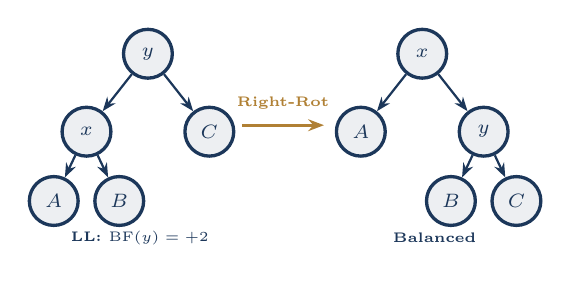
\begin{tikzpicture}[x=0.52cm,y=0.55cm]
  \node[avlnode] (y) at (1.5,1.8) {$y$};
  \node[avlnode] (x) at (0,0) {$x$};
  \node[avlnode] (c) at (3,0) {$C$};
  \node[avlnode] (a) at (-0.8,-1.6) {$A$};
  \node[avlnode] (b) at (0.8,-1.6) {$B$};
  \draw[avledge] (y)--(x); \draw[avledge] (y)--(c);
  \draw[avledge] (x)--(a); \draw[avledge] (x)--(b);
  \node[font=\tiny\bfseries\color{primary}] at (1.3,-2.45) {LL: $\bfactor{y}=+2$};
  \draw[-{Stealth[length=2mm]},very thick,accent] (3.8,0.15) -- (5.8,0.15) node[midway,above=2pt,font=\tiny\bfseries\color{accent}]{Right-Rot};
  \node[avlnode] (xx) at (8.2,1.8) {$x$};
  \node[avlnode] (aa) at (6.7,0) {$A$};
  \node[avlnode] (yy) at (9.7,0) {$y$};
  \node[avlnode] (bb) at (8.9,-1.6) {$B$};
  \node[avlnode] (cc) at (10.5,-1.6) {$C$};
  \draw[avledge] (xx)--(aa); \draw[avledge] (xx)--(yy);
  \draw[avledge] (yy)--(bb); \draw[avledge] (yy)--(cc);
  \node[font=\tiny\bfseries\color{primary}] at (8.5,-2.45) {Balanced};
\end{tikzpicture}
\end{column}

\begin{column}{0.50\textwidth}
\begin{block}{\footnotesize Algorithm: $\id{Rebalance\text{-}AVL}(v)$}
\scriptsize
\begin{tabular}{@{}p{0.42cm}>{\raggedright\arraybackslash}p{0.88\linewidth}@{}}
1. & Update $h(v)$ and $\bfactor{v} \gets h(v.\id{left}) - h(v.\id{right})$. \\
2. & \kw{if} $\bfactor{v} > 1$ \kw{then} \hfill $\triangleright$ Left-heavy \\
3. & \quad \kw{if} $\bfactor{v.\id{left}} < 0$ \kw{then} $v.\id{left} \gets \id{Left\text{-}Rotate}(v.\id{left})$ \\
4. & \quad \kw{return} $\id{Right\text{-}Rotate}(v)$ \\
5. & \kw{if} $\bfactor{v} < -1$ \kw{then} \hfill $\triangleright$ Right-heavy \\
6. & \quad \kw{if} $\bfactor{v.\id{right}} > 0$ \kw{then} $v.\id{right} \gets \id{Right\text{-}Rotate}(v.\id{right})$ \\
7. & \quad \kw{return} $\id{Left\text{-}Rotate}(v)$ \\
8. & \kw{return} $v$
\end{tabular}
\end{block}
\end{column}
\end{columns}
\end{frame}

\begin{frame}{Splay Tree (\texttt{splay\_tree.h}): Splaying, Split \& Join}
\begin{itemize}\setlength{\itemsep}{0.35em}\footnotesize
  \item \textbf{Three Splaying Rotation Types} (move accessed node $x$ to root):
  \[
    \textbf{\color{primary}Zig} \text{ (at root)} \qquad\quad
    \textbf{\color{primary}Zig-Zig} \text{ (same-side: rotate } g \text{ then } p\text{)} \qquad\quad
    \textbf{\color{primary}Zig-Zag} \text{ (opposite-side: rotate } p \text{ then } g\text{)}
  \]
\end{itemize}

\begin{columns}[T,onlytextwidth]
\begin{column}{0.48\textwidth}
\begin{block}{\footnotesize Split-Based $\id{Splay\text{-}Insert}(r, k)$}
\footnotesize
\begin{enumerate}\setlength{\itemsep}{0.3em}
  \item $r \gets \id{Splay}(r, k)$; if $r.\id{key} = k$, return $r$.
  \item Allocate new root $z$ with key $k$.
  \item Split $r$ around $k$ into $z.\id{left}$ and $z.\id{right}$.
\end{enumerate}
\end{block}
\end{column}

\begin{column}{0.48\textwidth}
\begin{exampleblock}{\footnotesize Join-Based $\id{Splay\text{-}Delete}(r, k)$}
\footnotesize
\begin{enumerate}\setlength{\itemsep}{0.3em}
  \item $r \gets \id{Splay}(r, k)$; if $r.\id{key} \neq k$, return $r$.
  \item Splay max of $r.\id{left}$: $r' \gets \id{Splay}(r.\id{left}, k)$.
  \item Join $r'.\id{right} \gets r.\id{right}$ and free $r$.
\end{enumerate}
\end{exampleblock}
\end{column}
\end{columns}
\end{frame}

\subsection{Red-Black Tree and Order-4 B+ Tree}
\begin{frame}{Red-Black Tree (\texttt{red\_black\_tree.h}): Fix-up Cases}
\begin{columns}[c,onlytextwidth]
\begin{column}{0.44\textwidth}
\begin{block}{\footnotesize Insertion Fix-up ($\le 2$ Rotations)}
\footnotesize
\begin{itemize}\setlength{\itemsep}{0.3em}
  \item \textbf{Case 1 (Red uncle $u$):} Recolor $p, u, g$; move up.
  \item \textbf{Case 2 (Black $u$, inner):} Rotate $p \to$ Case 3.
  \item \textbf{Case 3 (Black $u$, outer):} Recolor \& rotate $g$.
\end{itemize}
\end{block}

\vspace{0.2em}
\begin{alertblock}{\footnotesize Deletion Fix-up ($\le 3$ Rotations)}
\footnotesize
\begin{itemize}\setlength{\itemsep}{0.3em}
  \item \textbf{Case 1:} Red sibling $w \to$ rotate $p$.
  \item \textbf{Case 2:} Black $w$ \& black nephews $\to$ recolor.
  \item \textbf{Case 3:} Red inner nephew $\to$ rotate $w$.
  \item \textbf{Case 4:} Red outer nephew $\to$ rotate $p$, done.
\end{itemize}
\end{alertblock}
\end{column}

\begin{column}{0.53\textwidth}
\centering
\scriptsize\textbf{\color{primary}Four Double-Black Deletion Cases}\\[0.3em]
\begin{tikzpicture}[x=0.48cm,y=0.42cm]
  % Case 1
  \node[rbblack]  (p1) at (1.2,1.5) {$p$};
  \node[rbdouble] (x1) at (0.2,0.2) {$x$};
  \node[rbred]    (w1) at (2.2,0.2) {$w$};
  \draw[avledge] (p1)--(x1); \draw[avledge] (p1)--(w1);
  \draw[-{Stealth[length=1.5mm]},thick,accent] (2.9,0.8) -- (4.1,0.8) node[midway,above,font=\tiny\bfseries]{C1};
  \node[rbblack]  (w2) at (5.3,1.5) {$w$};
  \node[rbred]    (p2) at (4.5,0.2) {$p$};
  \node[rbblack]  (d2) at (6.1,0.2) {$d$};
  \draw[avledge] (w2)--(p2); \draw[avledge] (w2)--(d2);

  % Case 2
  \node[rbany]    (bp1) at (9.2,1.5) {$p$};
  \node[rbdouble] (bx1) at (8.2,0.2) {$x$};
  \node[rbblack]  (bw1) at (10.2,0.2) {$w$};
  \draw[avledge] (bp1)--(bx1); \draw[avledge] (bp1)--(bw1);
  \draw[-{Stealth[length=1.5mm]},thick,accent] (10.9,0.8) -- (12.1,0.8) node[midway,above,font=\tiny\bfseries]{C2};
  \node[rbdouble] (bp2) at (13.3,1.5) {$p$};
  \node[rbblack]  (bx2) at (12.5,0.2) {$x$};
  \node[rbred]    (bw2) at (14.1,0.2) {$w$};
  \draw[avledge] (bp2)--(bx2); \draw[avledge] (bp2)--(bw2);

  % Case 3
  \node[rbany]    (cp1) at (1.2,-2.2) {$p$};
  \node[rbdouble] (cx1) at (0.2,-3.5) {$x$};
  \node[rbblack]  (cw1) at (2.2,-3.5) {$w$};
  \node[rbred]    (cc1) at (1.6,-4.8) {$c$};
  \draw[avledge] (cp1)--(cx1); \draw[avledge] (cp1)--(cw1); \draw[avledge] (cw1)--(cc1);
  \draw[-{Stealth[length=1.5mm]},thick,accent] (2.9,-3.2) -- (4.1,-3.2) node[midway,above,font=\tiny\bfseries]{C3};
  \node[rbany]    (cp2) at (5.3,-2.2) {$p$};
  \node[rbdouble] (cx2) at (4.5,-3.5) {$x$};
  \node[rbblack]  (cc2) at (6.1,-3.5) {$c$};
  \node[rbred]    (cw2) at (6.7,-4.8) {$w$};
  \draw[avledge] (cp2)--(cx2); \draw[avledge] (cp2)--(cc2); \draw[avledge] (cc2)--(cw2);

  % Case 4
  \node[rbany]    (dp1) at (9.2,-2.2) {$p$};
  \node[rbdouble] (dx1) at (8.2,-3.5) {$x$};
  \node[rbblack]  (dw1) at (10.2,-3.5) {$w$};
  \node[rbred]    (dd1) at (10.8,-4.8) {$d$};
  \draw[avledge] (dp1)--(dx1); \draw[avledge] (dp1)--(dw1); \draw[avledge] (dw1)--(dd1);
  \draw[-{Stealth[length=1.5mm]},thick,accent] (10.9,-3.2) -- (12.1,-3.2) node[midway,above,font=\tiny\bfseries]{C4};
  \node[rbany]    (dw2) at (13.3,-2.2) {$w$};
  \node[rbblack]  (dp2) at (12.5,-3.5) {$p$};
  \node[rbblack]  (dd2) at (14.1,-3.5) {$d$};
  \node[rbblack]  (dx2) at (11.9,-4.8) {$x$};
  \draw[avledge] (dw2)--(dp2); \draw[avledge] (dw2)--(dd2); \draw[avledge] (dp2)--(dx2);
\end{tikzpicture}
\end{column}
\end{columns}
\end{frame}

\begin{frame}{Order-$4$ $\text{B}^+$ Tree (\texttt{B\_plus\_tree.h}): Split, Borrow \& Merge}
\begin{itemize}\setlength{\itemsep}{0.35em}\footnotesize
  \item \textbf{Structure ($M = 4$):} All data keys reside in linked leaves ($2\text{--}3$ keys); internal nodes store $1\text{--}3$ routing separators $\id{key}[i] = \min(\id{child}[i+1])$.
\end{itemize}

\vspace{0.2em}
\begin{columns}[T,onlytextwidth]
\begin{column}{0.48\textwidth}
\begin{block}{\footnotesize Insertion: Overflow Split}
\footnotesize
\begin{itemize}\setlength{\itemsep}{0.35em}
  \item \textbf{Leaf Overflow ($4$ keys):} Split into $2 + 2$ keys and link via \code{next}.
  \item \textbf{Internal Overflow ($5$ children):} Split into $3 + 2$ children and propagate upward.
\end{itemize}
\end{block}
\end{column}

\begin{column}{0.48\textwidth}
\begin{exampleblock}{\footnotesize Deletion: Underflow Borrow / Merge}
\footnotesize
\begin{itemize}\setlength{\itemsep}{0.35em}
  \item \textbf{Sibling Borrow:} Transfer boundary key/child if adjacent sibling has $>2$ keys.
  \item \textbf{Sibling Merge:} Merge underfull node with sibling and pull parent separator.
\end{itemize}
\end{exampleblock}
\end{column}
\end{columns}
\end{frame}

% ============================================================
%  SECTION 3: TESTING RESULTS
% ============================================================
\section{Testing Results}

\subsection{Functional Verification and Topologies}
\begin{frame}{Test Suite \& Structural Topology Verification}
\begin{columns}[b,onlytextwidth]
\begin{column}{0.18\textwidth}
\centering
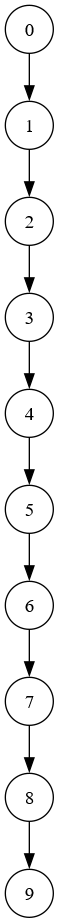
\includegraphics[height=2.2cm,keepaspectratio]{bst.png}\\
{\scriptsize \textbf{(a) BST}\\Right chain}
\end{column}
\begin{column}{0.18\textwidth}
\centering
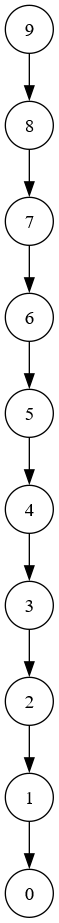
\includegraphics[height=2.2cm,keepaspectratio]{splay.png}\\
{\scriptsize \textbf{(b) Splay}\\Left chain}
\end{column}
\begin{column}{0.30\textwidth}
\centering
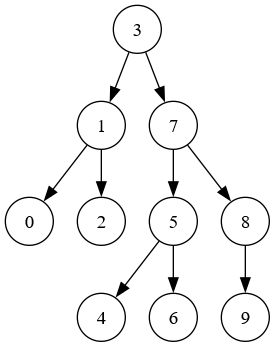
\includegraphics[width=\textwidth,height=2.2cm,keepaspectratio]{avl.png}\\
{\scriptsize \textbf{(c) AVL Tree}\\Height-balanced ($0..9$)}
\end{column}
\begin{column}{0.30\textwidth}
\centering
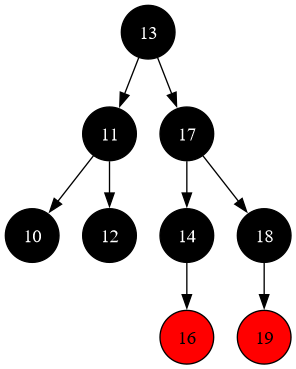
\includegraphics[width=\textwidth,height=2.2cm,keepaspectratio]{rb.png}\\
{\scriptsize \textbf{(d) Red-Black Tree}\\Keys $10..19$, delete $15$}
\end{column}
\end{columns}

\vspace{0.3em}
\begin{center}
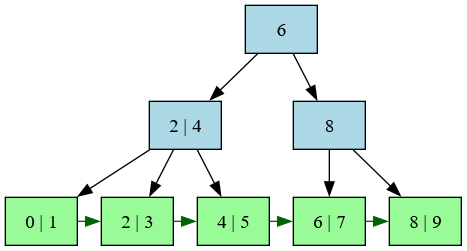
\includegraphics[width=0.65\textwidth,height=1.85cm,keepaspectratio]{b_plus.png}\\[0.1em]
{\scriptsize \textbf{(e) Order-$4$ $\text{B}^+$ Tree:} Internal separator nodes (blue) and linked data leaves (green)}
\end{center}
\end{frame}

\subsection{Benchmark Timings and Curves}
\begin{frame}{Execution Time Summary Table (in Milliseconds)}
\centering
\renewcommand{\arraystretch}{0.92}
\setlength{\tabcolsep}{5pt}
\tiny
\begin{tabular}{@{}llrrrrrr@{}}
\toprule
\textbf{\color{primary}Scenario} & \textbf{\color{primary}Tree} & \textbf{\color{primary}$N=1{,}000$} & \textbf{\color{primary}$N=10{,}000$} & \textbf{\color{primary}$N=20{,}000$} & \textbf{\color{primary}$N=30{,}000$} & \textbf{\color{primary}$N=40{,}000$} & \textbf{\color{primary}$N=50{,}000$} \\
\midrule
\multirow{5}{*}{\shortstack[l]{Scenario 1: Ordered\\Insertion (ms)}}
  & BST       & 0.754 & 69.678 & 264.054 & 628.587 & 1129.765 & \textbf{\color{Red3}1888.738} \\
  & AVL       & 0.183 &  1.702 &   2.992 &   4.424 &    6.619 &    7.833 \\
  & Splay     & 0.036 &  0.250 &   0.581 &   0.514 &    0.736 & \textbf{\color{progcolor}0.778} \\
  & Red-Black & 0.136 &  1.210 &   2.590 &   3.873 &    5.615 &    6.942 \\
  & $\text{B}^+$ Tree & 0.247 &  2.972 &   4.557 &   6.809 &    8.891 &   12.355 \\
\midrule
\multirow{5}{*}{\shortstack[l]{Scenario 1: Ordered\\Deletion (ms)}}
  & BST       & 0.016 &  0.171 &   0.217 &   0.301 &    0.399 & \textbf{\color{progcolor}0.599} \\
  & AVL       & 0.130 &  1.069 &   2.221 &   4.712 &    5.656 &    8.075 \\
  & Splay     & 0.044 &  0.227 &   0.449 &   0.735 &    0.929 &    1.177 \\
  & Red-Black & 0.054 &  0.485 &   1.021 &   1.609 &    2.931 &    3.319 \\
  & $\text{B}^+$ Tree & 0.159 &  1.332 &   3.167 &   6.714 &    9.338 &   12.306 \\
\midrule
\multirow{5}{*}{\shortstack[l]{Scenario 2: Reverse\\Deletion (ms)}}
  & BST       & 0.684 & 63.698 & 251.397 & 590.257 & 1139.824 & \textbf{\color{Red3}1777.648} \\
  & AVL       & 0.121 &  1.130 &   2.412 &   4.375 &    5.891 &    8.341 \\
  & Splay     & 0.018 &  0.110 &   0.227 &   0.336 &    0.391 & \textbf{\color{progcolor}0.646} \\
  & Red-Black & 0.071 &  0.522 &   1.059 &   2.438 &    2.246 &    3.177 \\
  & $\text{B}^+$ Tree & 0.157 &  1.281 &   3.182 &   5.975 &    6.615 &    8.095 \\
\midrule
\multirow{5}{*}{\shortstack[l]{Scenario 3: Random\\Insertion (ms)}}
  & BST       & 0.090 &  0.843 &   1.941 &   3.838 &    4.015 & \textbf{\color{progcolor}5.524} \\
  & AVL       & 0.334 &  2.155 &   4.478 &   9.397 &   10.925 &   12.785 \\
  & Splay     & 0.166 &  1.858 &   3.941 &   7.184 &    8.619 &   10.446 \\
  & Red-Black & 0.179 &  1.588 &   3.563 &   5.608 &    7.387 &   10.409 \\
  & $\text{B}^+$ Tree & 0.276 &  3.000 &   7.625 &  12.549 &   16.264 &   19.595 \\
\midrule
\multirow{5}{*}{\shortstack[l]{Scenario 3: Random\\Deletion (ms)}}
  & BST       & 0.074 &  0.764 &   1.753 &   2.985 &    4.417 & \textbf{\color{progcolor}5.359} \\
  & AVL       & 0.276 &  1.851 &   4.748 &   7.178 &   10.779 &   13.538 \\
  & Splay     & 0.198 &  1.371 &   3.342 &   6.337 &    7.656 &   10.079 \\
  & Red-Black & 0.239 &  1.095 &   2.456 &   4.473 &    5.650 &    7.303 \\
  & $\text{B}^+$ Tree & 0.235 &  2.548 &   6.142 &  11.828 &   16.430 &   20.871 \\
\bottomrule
\end{tabular}
\end{frame}

\begin{frame}{Runtime Curves: Scenario 1 \& Scenario 2 (Monotone Inputs)}
\begin{columns}[c,onlytextwidth]
\begin{column}{0.32\textwidth}
\centering
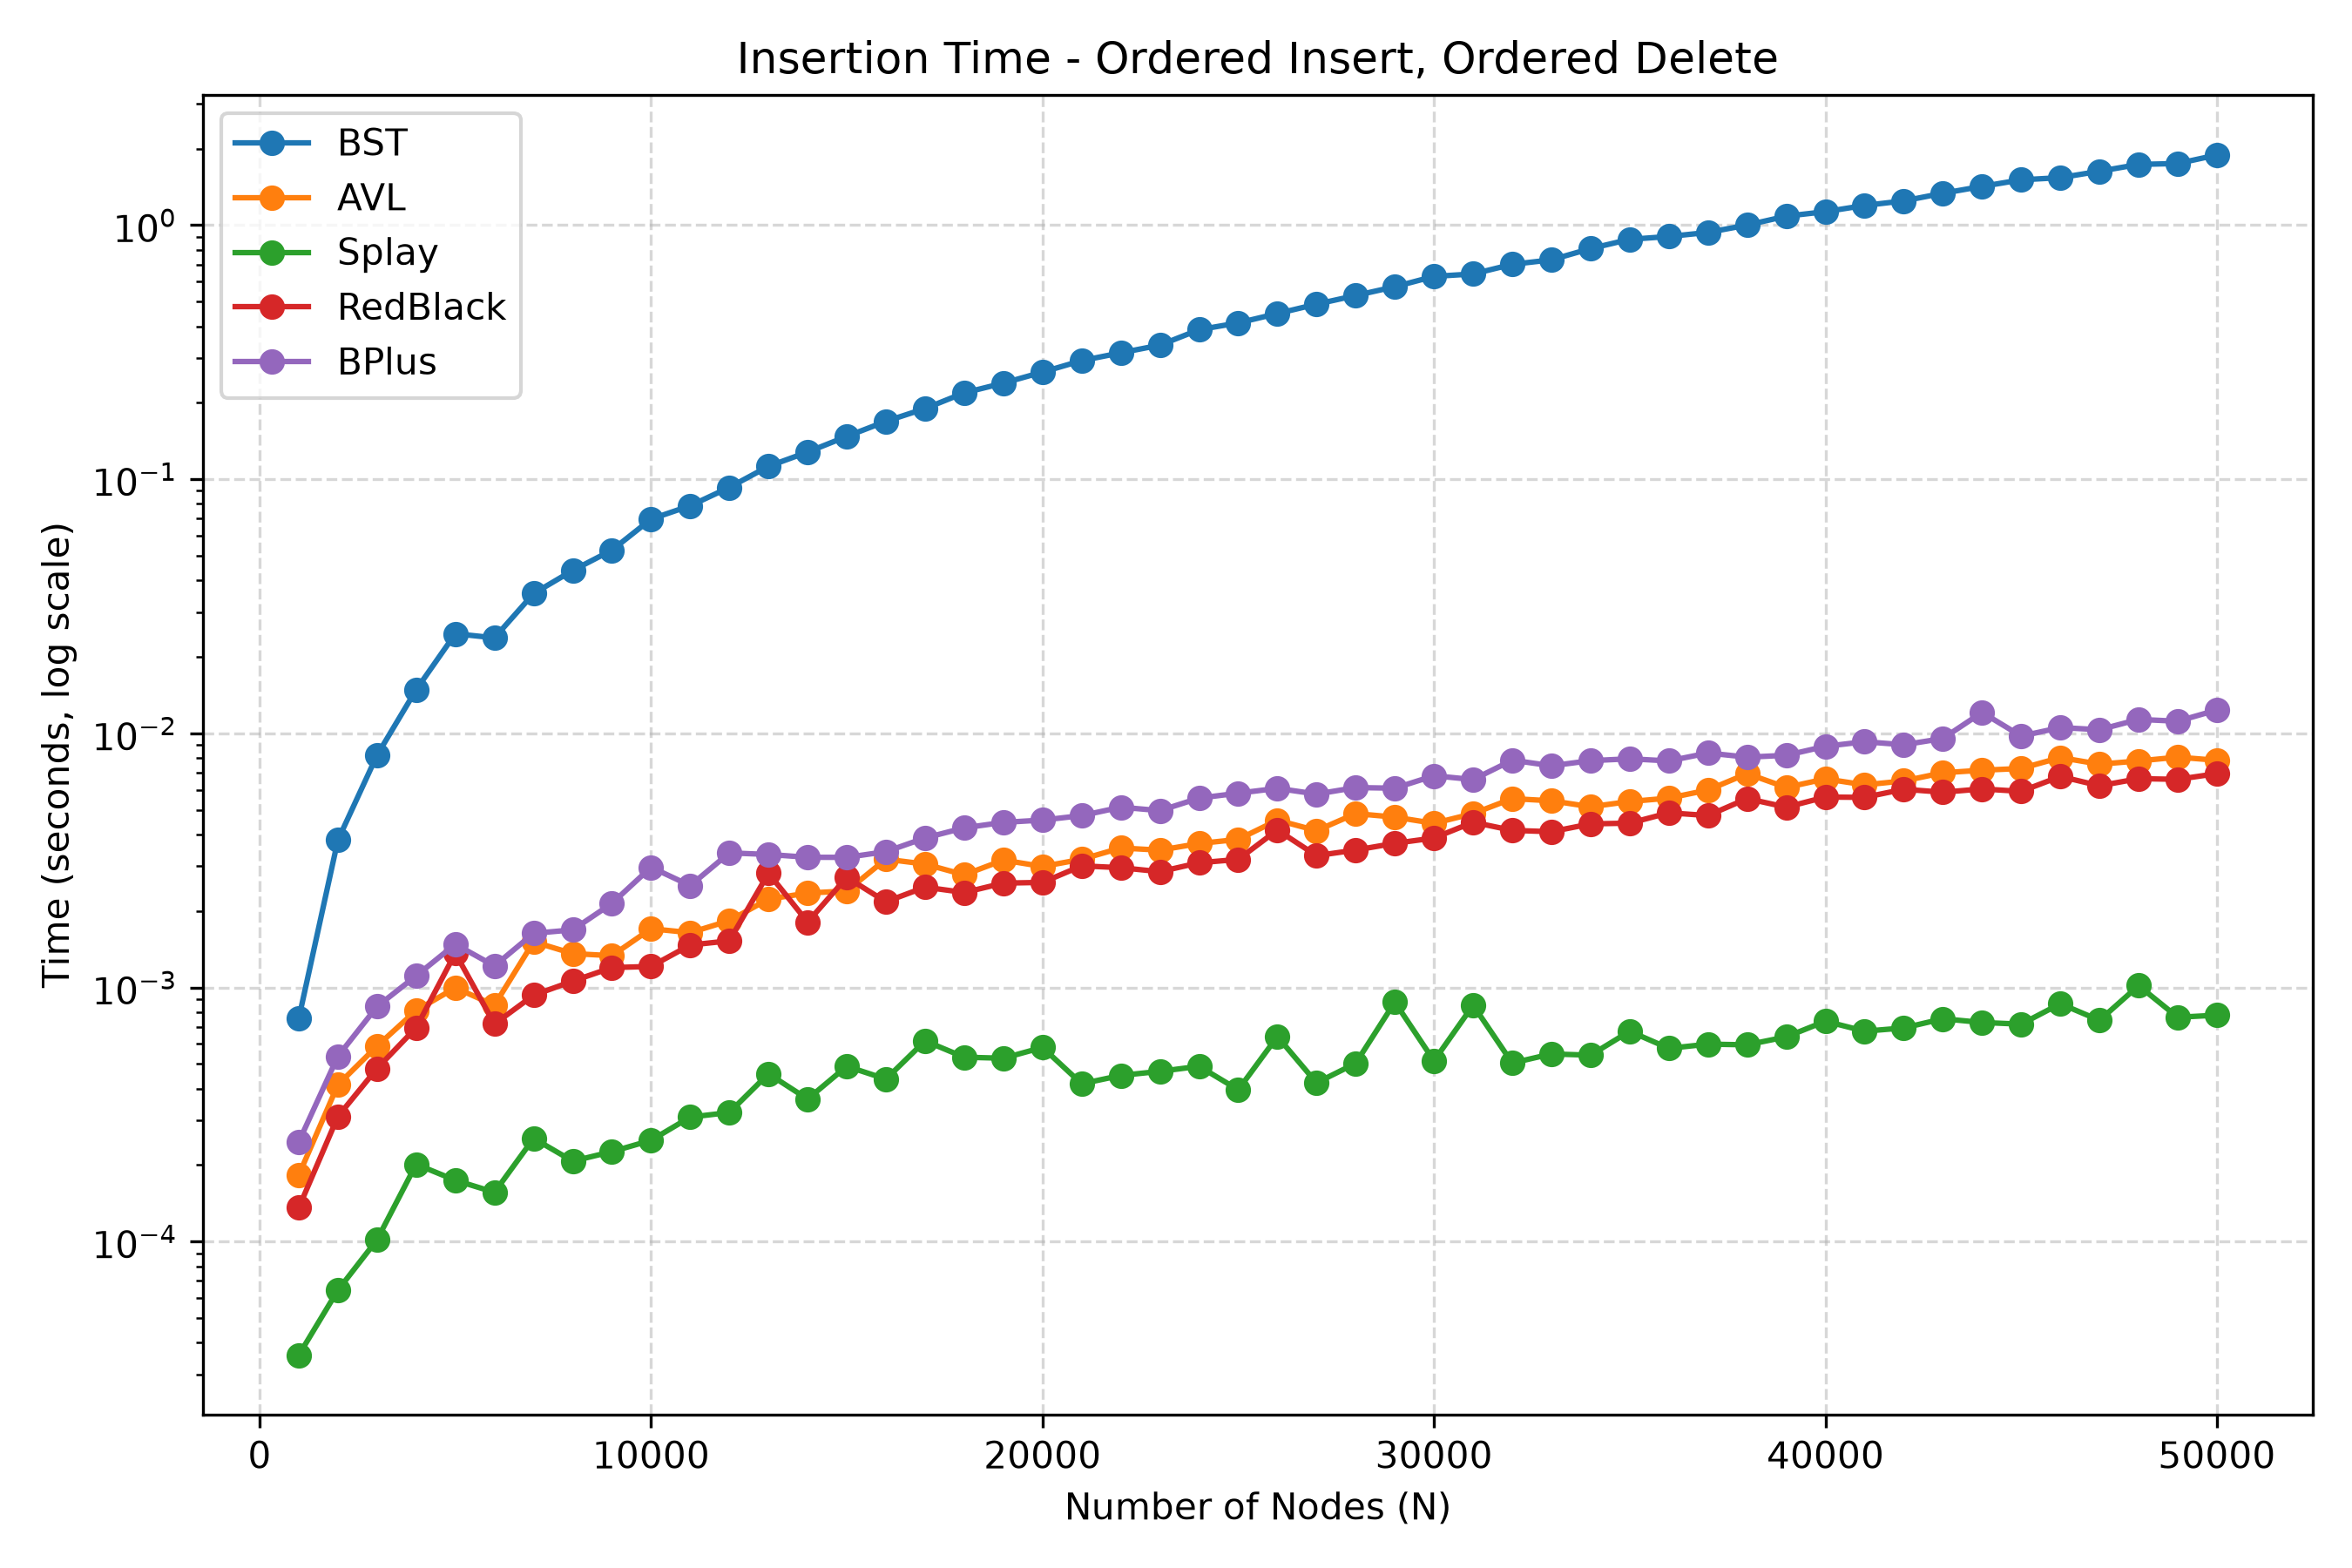
\includegraphics[width=\linewidth]{ordered_insert_seconds.png}\\
{\scriptsize (a) Ordered Insert}
\end{column}
\begin{column}{0.32\textwidth}
\centering
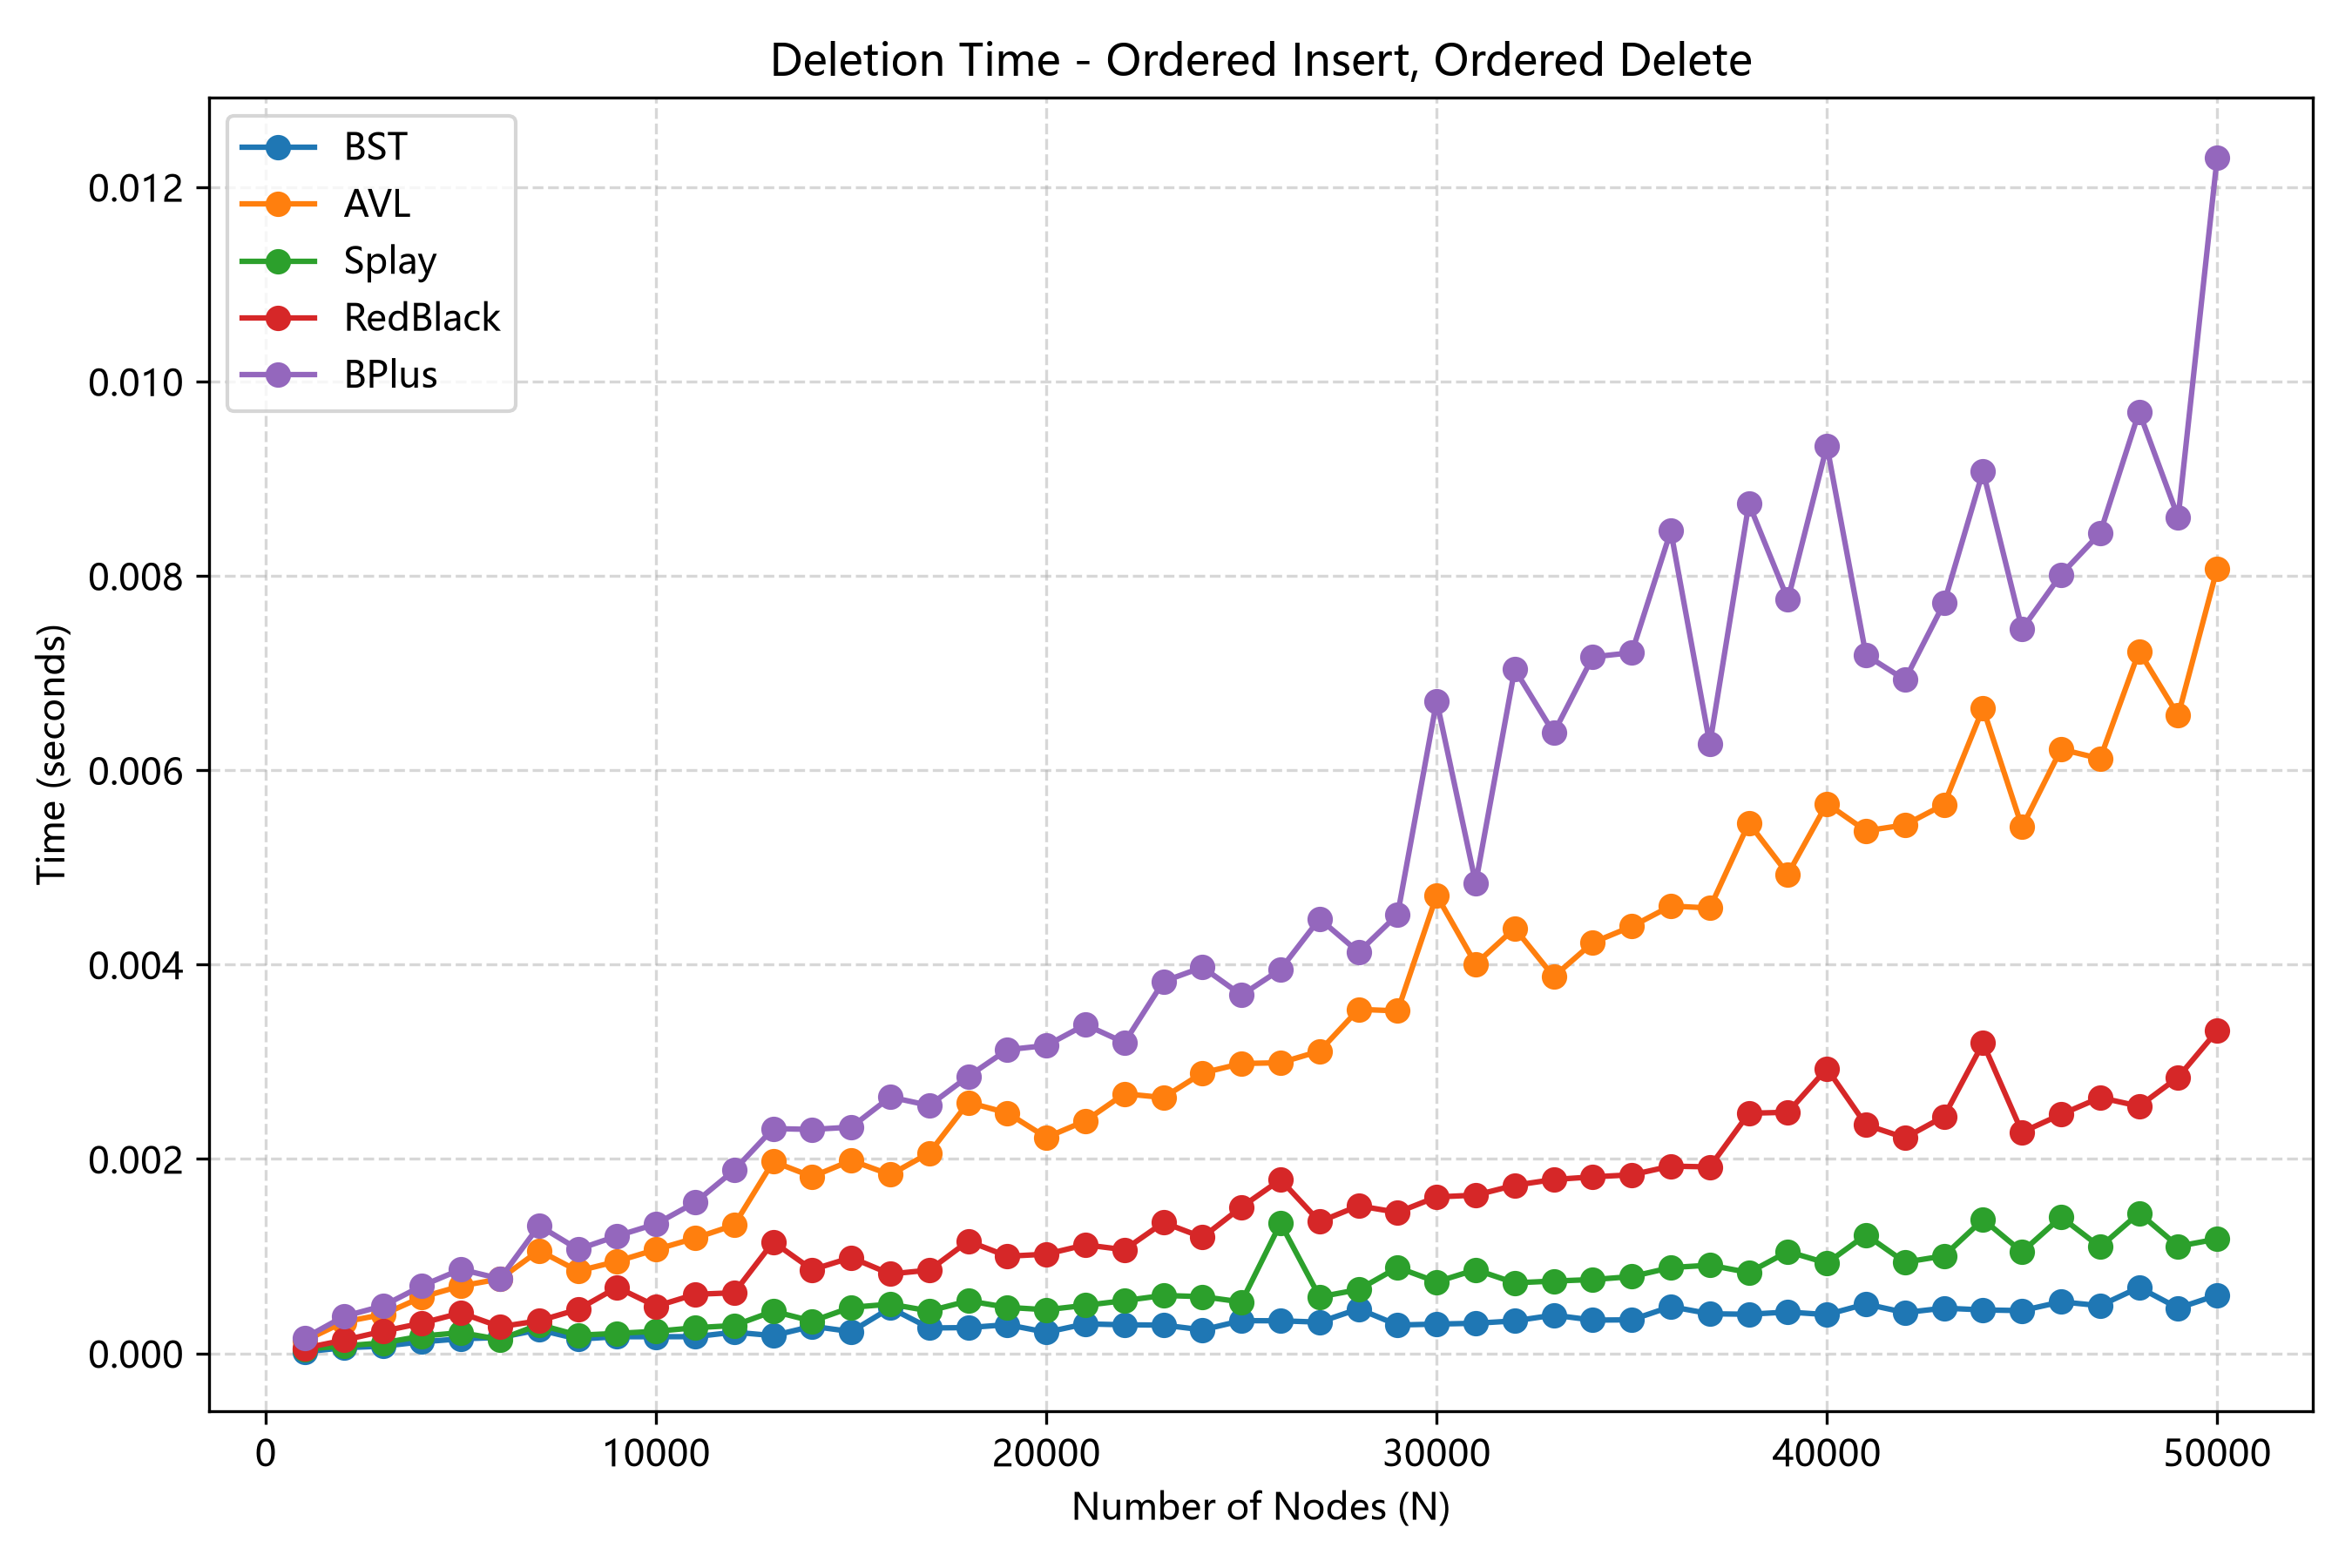
\includegraphics[width=\linewidth]{ordered_delete_seconds.png}\\
{\scriptsize (b) Scenario 1: Same-Order Delete}
\end{column}
\begin{column}{0.32\textwidth}
\centering
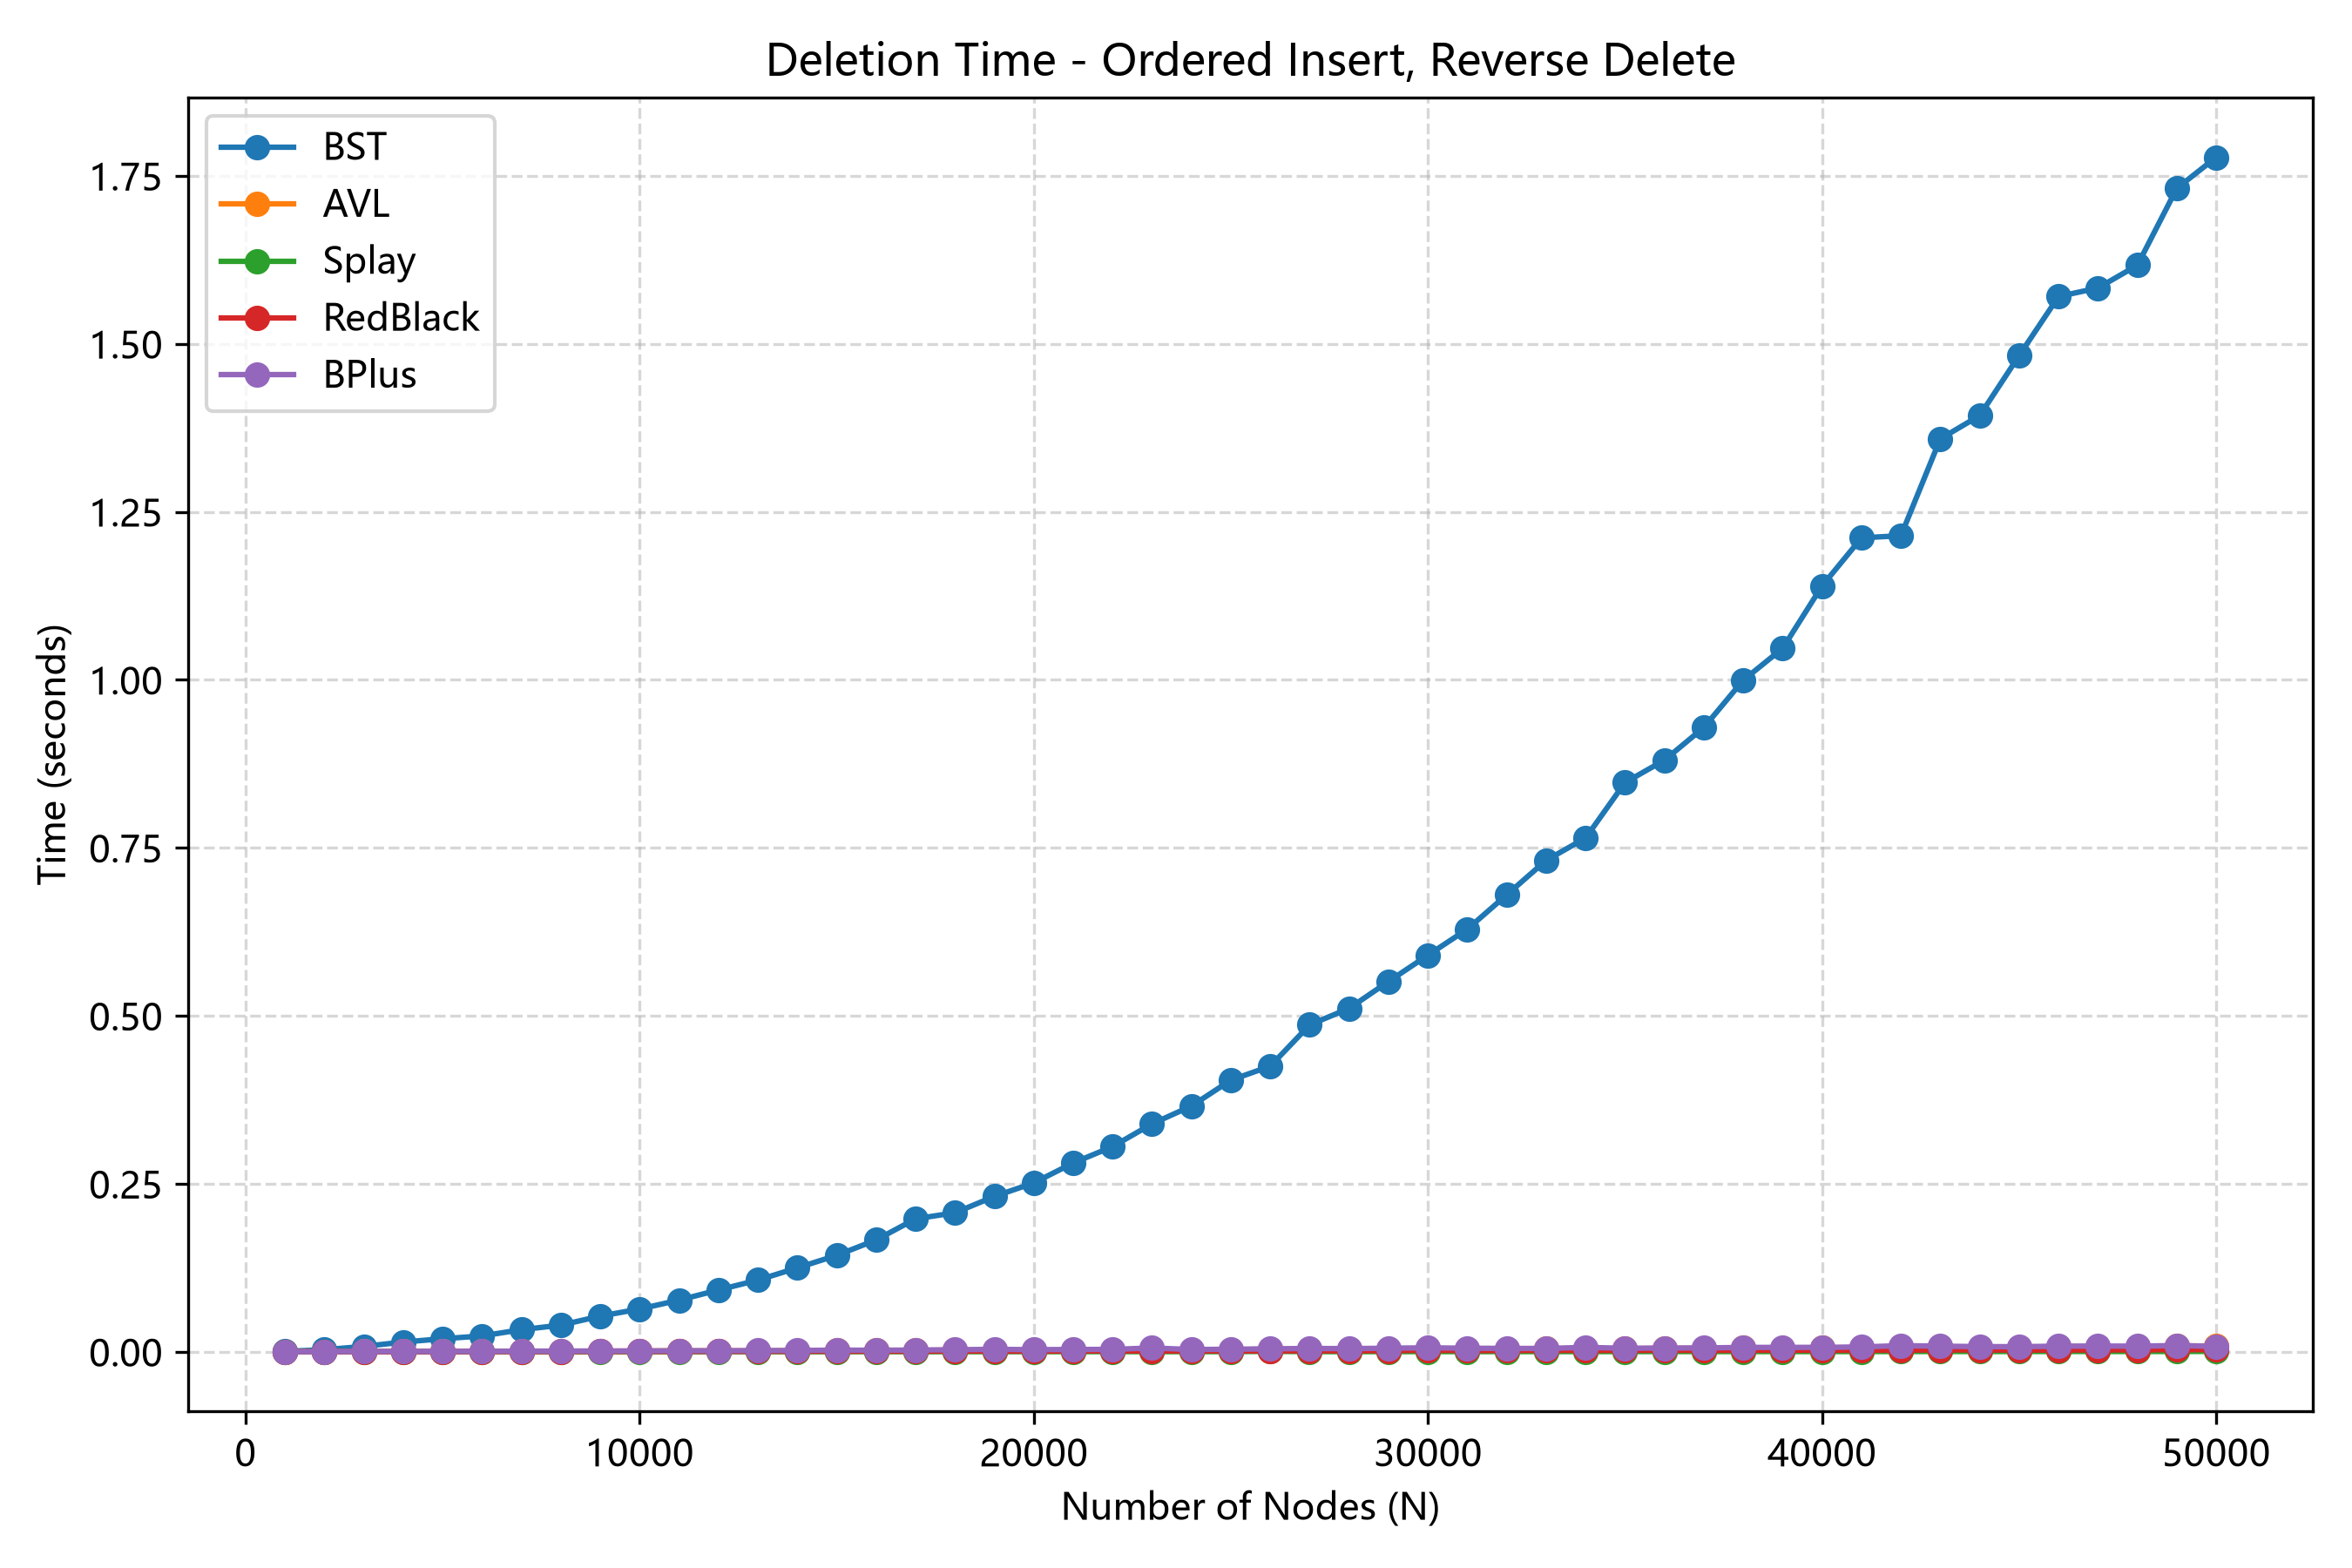
\includegraphics[width=\linewidth]{ordered_reverse_delete_seconds.png}\\
{\scriptsize (c) Scenario 2: Reverse Delete}
\end{column}
\end{columns}

\vspace{0.4em}
\begin{itemize}\footnotesize\setlength{\itemsep}{0.25em}
  \item \textbf{Unbalanced BST:} $\Theta(N^2)$ on ordered insert ($1.89\,\text{s}$) and reverse delete ($1.78\,\text{s}$), but $\Theta(N)$ on same-order delete ($0.60\,\text{ms}$).
  \item \textbf{Splay Tree:} Fastest on sorted insert ($0.78\,\text{ms}$) and reverse delete ($0.65\,\text{ms}$).
\end{itemize}
\end{frame}

\begin{frame}{Runtime Curves: Scenario 3 (Random Insert + Random Delete)}
\begin{columns}[c,onlytextwidth]
\begin{column}{0.47\textwidth}
\centering
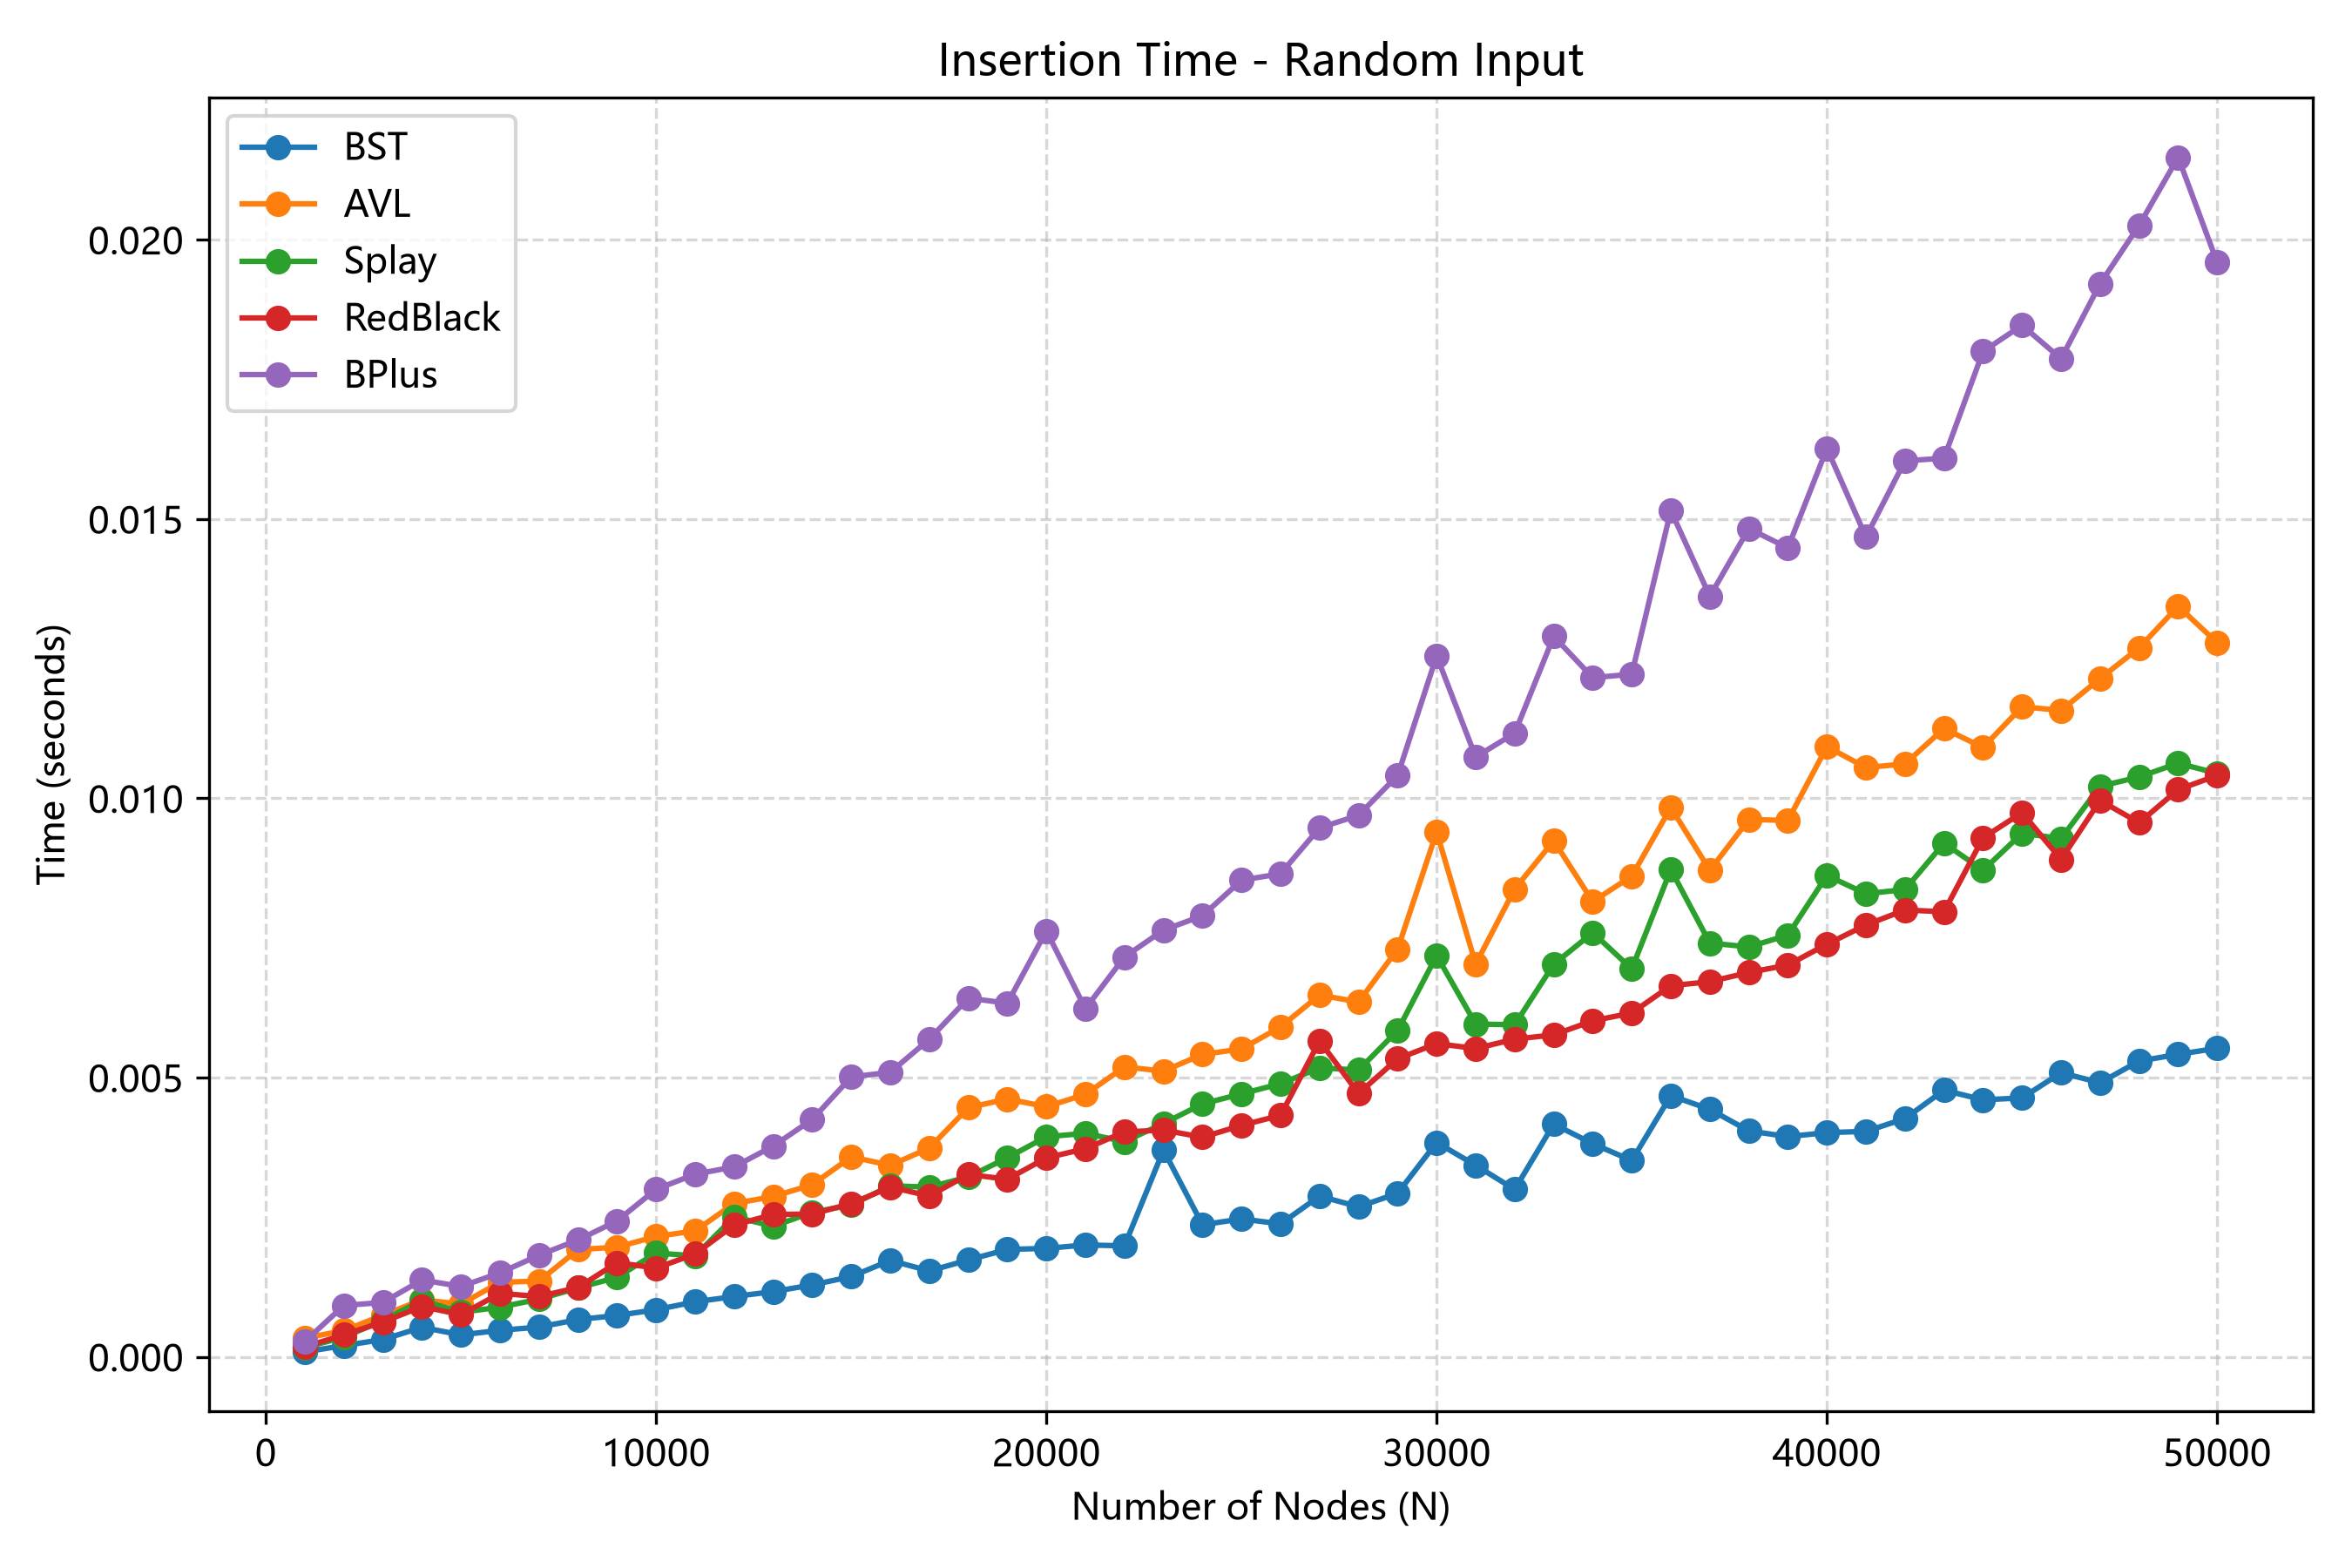
\includegraphics[width=\linewidth]{random_insert_seconds.png}\\
{\scriptsize (a) Random Insertion Time}
\end{column}
\begin{column}{0.47\textwidth}
\centering
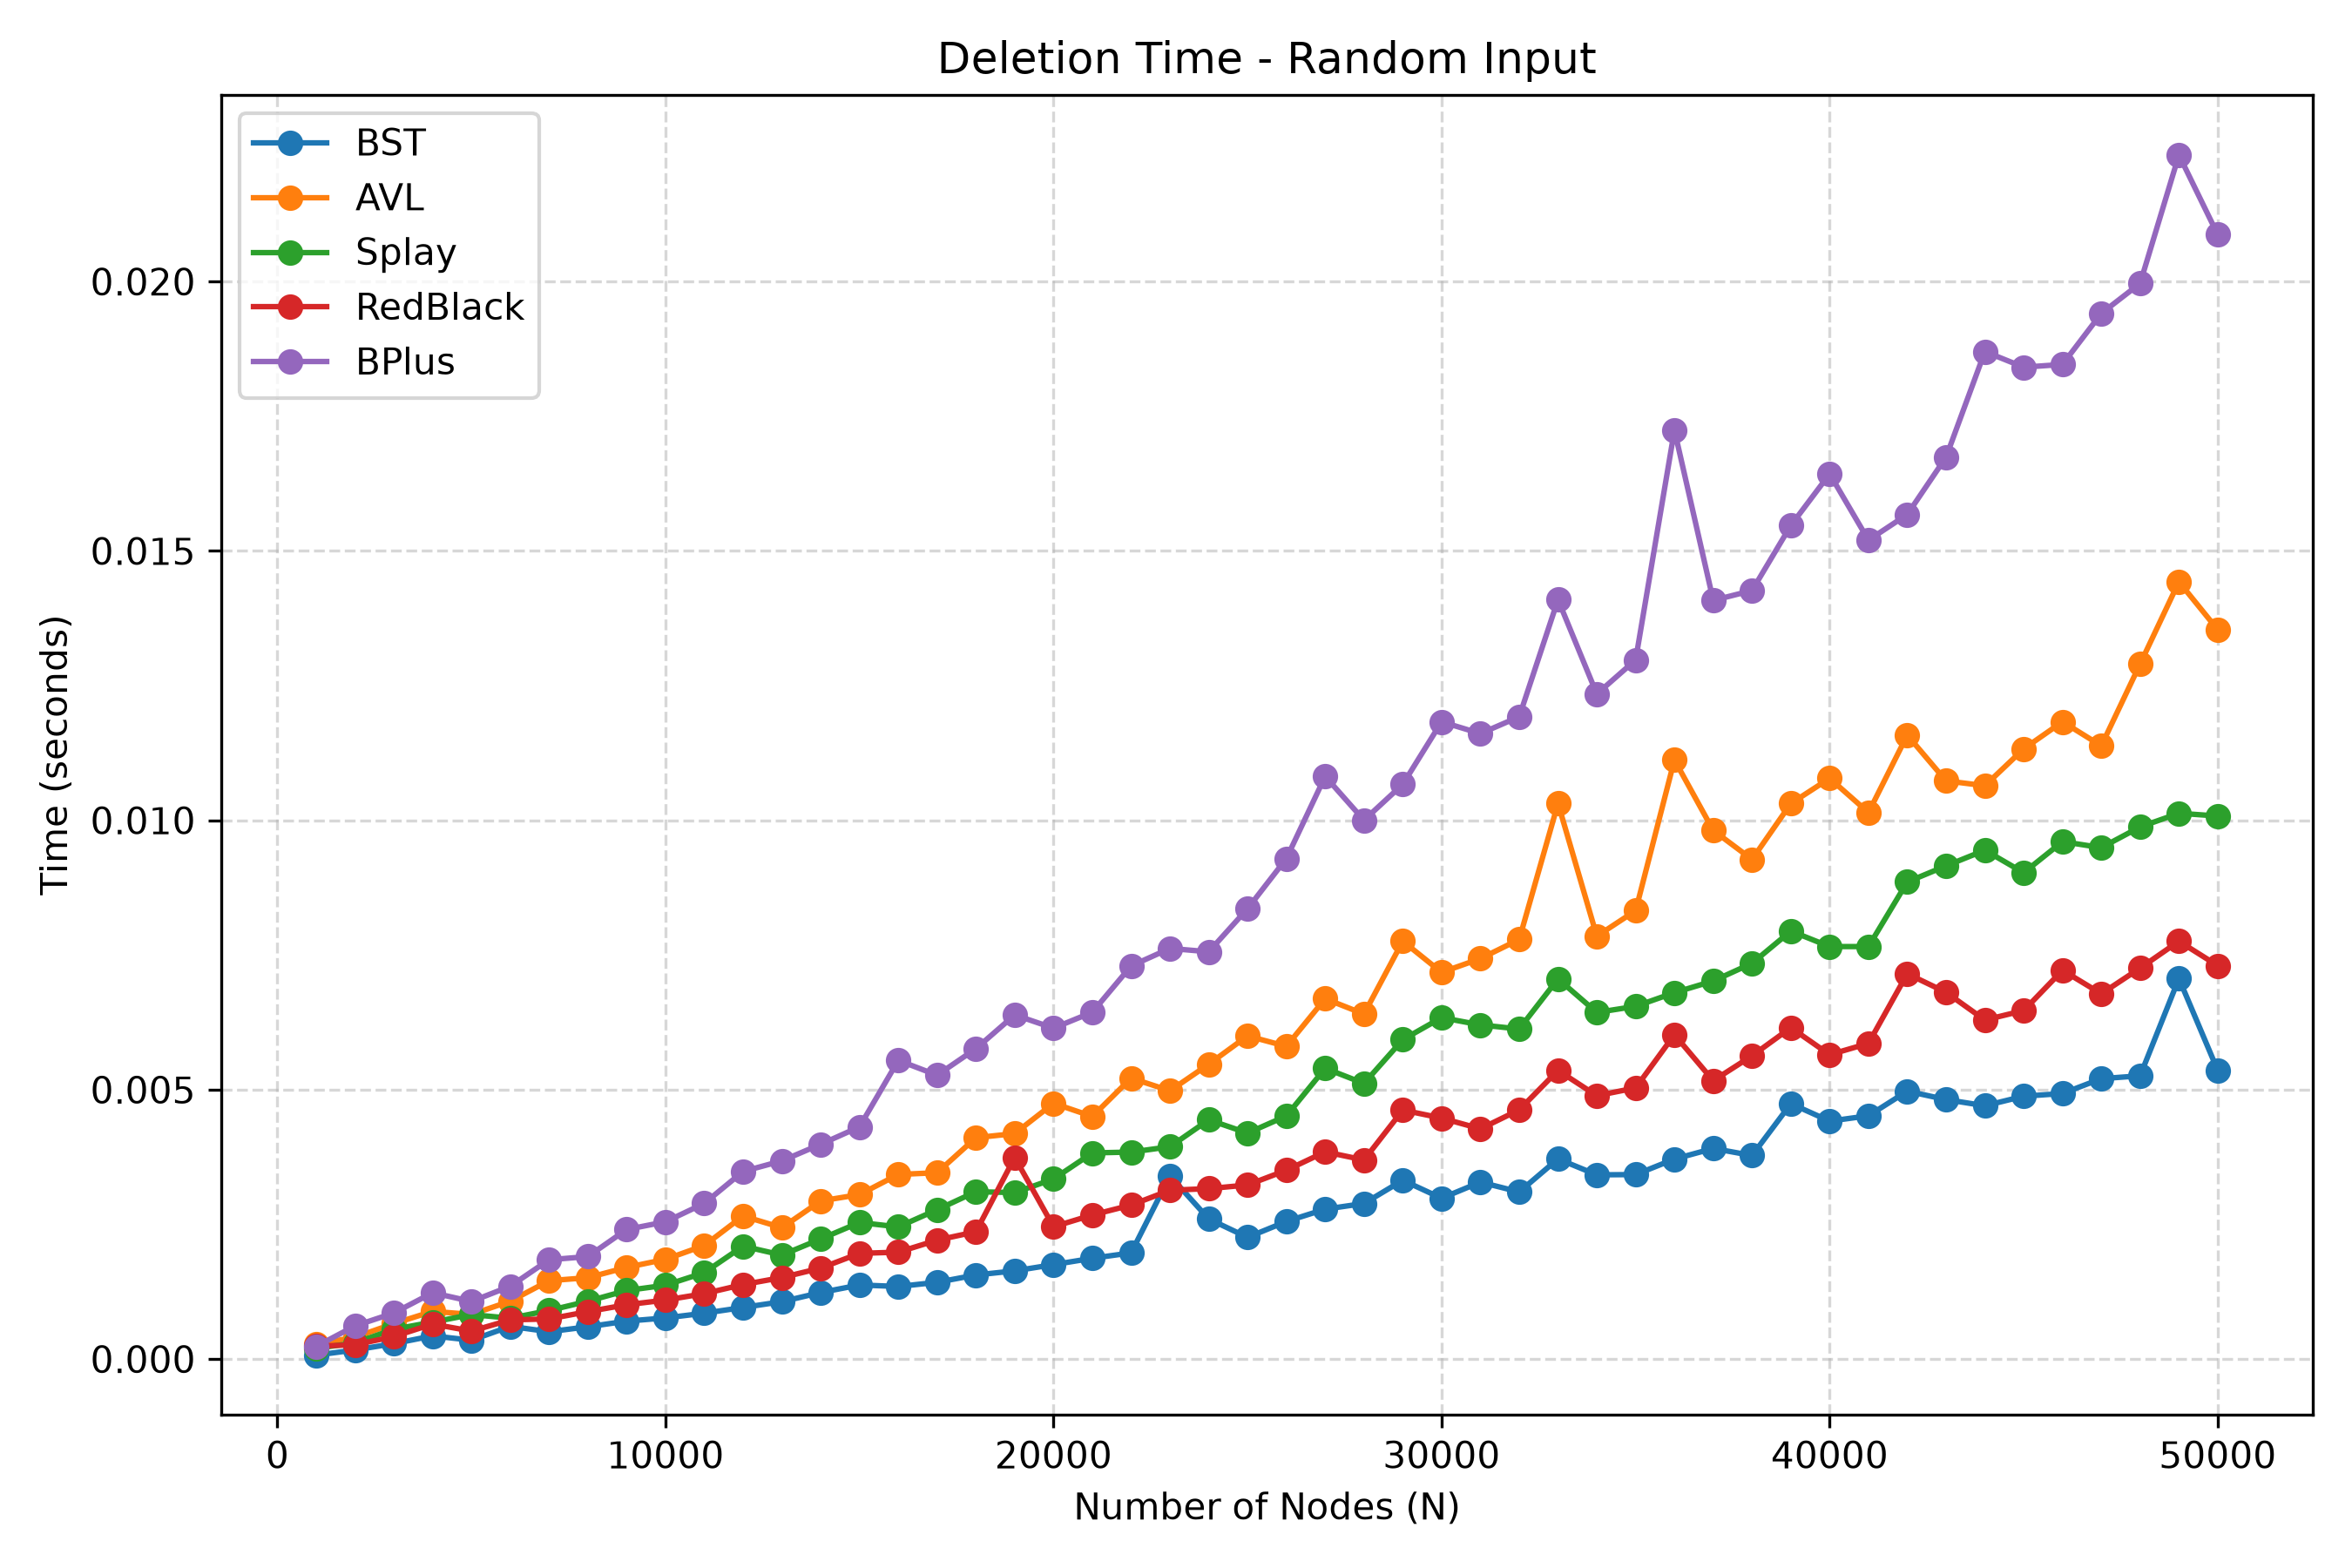
\includegraphics[width=\linewidth]{random_delete_seconds.png}\\
{\scriptsize (b) Random Deletion Time}
\end{column}
\end{columns}

\vspace{0.3em}
\begin{itemize}\footnotesize
  \item All five trees scale as $\Theta(N\log N)$ under random inputs ($< 21\,\text{ms}$ at $N = 50{,}000$).
  \item Ranking: $\textbf{BST} < \textbf{Red-Black} < \textbf{Splay} < \textbf{AVL} < \textbf{B}^+\textbf{ Tree}$.
\end{itemize}
\end{frame}

% ============================================================
%  SECTION 4: ANALYSIS AND COMMENTS
% ============================================================
\section{Analysis and Comments}

\subsection{Time and Space Complexity}
\begin{frame}{Asymptotic Time \& Space Complexity Comparison}
\renewcommand{\arraystretch}{1.18}
\scriptsize
\begin{tabular}{@{}lccccc@{}}
\toprule
\textbf{\color{primary}Structure} & \textbf{\color{primary}Avg Op} & \textbf{\color{primary}Worst Op} & \textbf{\color{primary}Scenario 1} & \textbf{\color{primary}Scenario 2} & \textbf{\color{primary}Node Size / Aux Stack} \\
\midrule
\textbf{Unbalanced BST}   & $\Theta(\log N)$ & $\Theta(N)$        & $\Theta(N^2)$ / $\Theta(N)$ & $\Theta(N^2)$ / $\Theta(N^2)$ & $24\,\text{B}$, $O(1)$ iterative \\
\textbf{AVL Tree}         & $\Theta(\log N)$ & $\Theta(\log N)$   & $\Theta(N\log N)$           & $\Theta(N\log N)$             & $32\,\text{B}$, $O(\log N)$ stack \\
\textbf{Splay Tree}       & $\Theta(\log N)$ amort. & $\Theta(N)$ & $\Theta(N)$ / $\Theta(N)$   & $\Theta(N)$ / $\Theta(N)$     & $24\,\text{B}$, $O(H)$ stack \\
\textbf{Red-Black Tree}   & $\Theta(\log N)$ & $\Theta(\log N)$   & $\Theta(N\log N)$           & $\Theta(N\log N)$             & $40\,\text{B}$, $O(1)$ iterative \\
\textbf{Order-$4$ $\text{B}^+$ Tree} & $\Theta(\log N)$ & $\Theta(\log N)$ & $\Theta(N\log N)$    & $\Theta(N\log N)$             & Dynamic arrays ($M=4$) \\
\bottomrule
\end{tabular}

\vspace{0.55em}
\begin{block}{\footnotesize Memory Layout Highlights (64-bit Target)}
\footnotesize
\begin{itemize}\setlength{\itemsep}{0.25em}
  \item \textbf{Binary Trees:} $24\text{--}40\,\text{bytes/node}$ depending on balance metadata (\code{height}/\code{BF} in AVL; \code{color}/\code{parent} in RB).
  \item \textbf{Order-$4$ $\text{B}^+$ Tree:} Each node allocates dynamic \code{keys[4]} and \code{children[5]} arrays, reducing tree depth to $\log_{2\dots 4} N$ at the cost of extra heap allocations.
\end{itemize}
\end{block}
\end{frame}

\subsection{Key Empirical Findings}
\begin{frame}{Finding 1: Asymmetry of Unbalanced BST Deletion}
\begin{alertblock}{Why Same-Order Delete Takes $0.60\,\text{ms}$ While Reverse Delete Takes $1.78\,\text{s}$?}
\footnotesize
After inserting $0, 1, \dots, N-1$, the BST is a right-skewed chain $0 \to 1 \to \dots \to N-1$:
\begin{itemize}\setlength{\itemsep}{0.45em}
  \item \textbf{Ordered Insertion ($\Theta(N^2)$, $1.89\,\text{s}$):} The $k$-th insertion walks $k$ nodes to the bottom leaf:
  \[
    \sum_{k=0}^{N-1} k = \frac{N(N-1)}{2} = \Theta(N^2) \quad (N\times 5 \implies 27.1\times \text{ runtime}).
  \]
  \item \textbf{Scenario 1 --- Increasing Delete ($\Theta(N)$, $0.60\,\text{ms}$):} Key $0, 1, \dots$ is always the \textbf{current root}, removed in $O(1)$ time via $\code{root} \gets \code{root->Right}$.
  \item \textbf{Scenario 2 --- Reverse Delete ($\Theta(N^2)$, $1.78\,\text{s}$):} Key $N-1, N-2, \dots$ is always the \textbf{deepest leaf}, requiring $N-k$ steps from the root on every deletion.
\end{itemize}
\end{alertblock}
\end{frame}

\begin{frame}{Finding 2: $\Theta(N)$ Sequential Locality of Splay Trees}
\begin{exampleblock}{Why Splay Tree Dominates Monotone Workloads ($< 1.2\,\text{ms}$ at $N=50{,}000$)}
\footnotesize
\begin{itemize}\setlength{\itemsep}{0.55em}
  \item \textbf{Increasing Insertion ($\Theta(N)$, $0.78\,\text{ms}$):} Each inserted key $k$ becomes the new root with an empty right subtree $\implies$ inserting $k+1$ terminates at the root in $O(1)$ time, forming a left-skewed spine $N-1 \to \dots \to 0$.
  \item \textbf{Reverse Deletion ($\Theta(N)$, $0.65\,\text{ms}$):} Deleting $N-1, N-2, \dots, 0$ repeatedly removes the current root of the left spine in $O(1)$ time.
  \item \textbf{Increasing Deletion ($\Theta(N)$ amortized, $1.18\,\text{ms}$):} The first \code{findSplay(root, 0)} performs \emph{zig-zig} rotations along the spine, \textbf{halving the depth of every node} and folding the chain into a shallow tree.
\end{itemize}
\end{exampleblock}
\end{frame}

\begin{frame}{Finding 3: Trade-offs Under Random Workloads}
At $N = 50{,}000$, uniform random updates yield:
{\footnotesize\[
\textbf{BST } (5.5\,\text{ms}) < \textbf{Red-Black } (10.4 / 7.3\,\text{ms}) < \textbf{Splay } (10.4 / 10.1\,\text{ms}) < \textbf{AVL } (12.8 / 13.5\,\text{ms}) < \textbf{B}^+ \text{ } (19.6 / 20.9\,\text{ms})
\]}

\begin{itemize}\setlength{\itemsep}{0.45em}\footnotesize
  \item \textbf{Unbalanced BST:} Expected depth $2\ln N \approx 1.39\log_2 N$ with zero rotation/metadata overhead.
  \item \textbf{Red-Black vs.\ AVL Tree:} Red-Black is \textbf{$20\%\text{--}45\%$ faster} ($\le 2$ insert / $\le 3$ delete rotations vs.\ up to $\Theta(\log N)$ AVL deletion rotations).
  \item \textbf{Splay Tree:} Loses sequential locality under uniform random access; pays continuous splaying overhead.
  \item \textbf{Order-$4$ $\text{B}^+$ Tree:} Highest CPU overhead in RAM due to small-node array shifting, \code{malloc} calls, and \code{refreshBPlusAncestors} traversal.
\end{itemize}
\end{frame}

\subsection{Further Improvements and Summary}
\begin{frame}{Further Improvements \& Practical Takeaways}
\begin{block}{\footnotesize Further Possible Engineering Improvements}
\footnotesize
\begin{enumerate}\setlength{\itemsep}{0.3em}
  \item \textbf{Cache Minimum Key in $\text{B}^+$ Nodes:} Avoid \code{refreshBPlusAncestors} walking down \code{children[0]} on every update.
  \item \textbf{Fixed-Size Arrays in $\text{B}^+$ Struct:} Embed \code{int keys[M]} and \code{BPlusTreeNode* children[M+1]} directly to eliminate extra \code{malloc} calls.
  \item \textbf{Top-Down Splaying \& Memory Pool:} Use iterative top-down splaying and a pre-allocated node memory pool (\textbf{from OOP Lab 7 last semester}).
\end{enumerate}
\end{block}

\vspace{0.25em}
\begin{exampleblock}{\footnotesize Summary: Choosing the Right Search Tree}
\footnotesize
\begin{itemize}\setlength{\itemsep}{0.25em}
  \item \textbf{Purely Random Keys:} Unbalanced BST (fastest constant factor, no worst-case protection).
  \item \textbf{Skewed / Sequential Locality:} Splay Tree ($\Theta(N)$ sequential performance).
  \item \textbf{General-Purpose Dictionary:} Red-Black Tree (best worst-case guarantee vs.\ rotation cost).
\end{itemize}
\end{exampleblock}
\end{frame}

% ============================================================
%  THANK YOU SLIDE
% ============================================================
\begin{frame}[plain]
\begin{tikzpicture}[remember picture, overlay]
    \fill[coverbg] (current page.south west) rectangle (current page.north east);
    \fill[primary] (current page.north west) rectangle ([yshift=-0.25cm]current page.north east);
    \fill[accent] ([yshift=-0.25cm]current page.north west) rectangle ([yshift=-0.34cm]current page.north east);
    \draw[accent!45, line width=0.7pt]
        ([xshift=1.1cm, yshift=-1.0cm]current page.north west) --
        ([xshift=1.1cm, yshift=1.0cm]current page.south west);
    \draw[accent!45, line width=0.7pt]
        ([xshift=-1.1cm, yshift=-1.0cm]current page.north east) --
        ([xshift=-1.1cm, yshift=1.0cm]current page.south east);
\end{tikzpicture}
\vfill
\begin{center}
    {\LARGE\bfseries\color{primary} Thank You for Listening!}\\[0.35cm]
    {\color{accent}\rule{0.28\textwidth}{1.0pt}}\\[0.45cm]
    {\large\color{primary}\textsf{Questions \& Discussion}}\\[0.7cm]
    {\normalsize\bfseries\color{primary} Yixiang Chen \hspace{2.5em} Runhui Lin}\\[0.18cm]
    {\footnotesize\color{textmuted} School of Mathematical Sciences, Zhejiang University}\\[0.1cm]
    {\scriptsize\color{textmuted} Advanced Data Structures and Algorithm Analysis $\cdot$ Fall--Winter 2026}
\end{center}
\vfill
\end{frame}

\end{document}
